\section{Case Studies}
\label{sec:cases}

We contrast three roles on three representative problems: a top proprietary agent (\textbf{codex + GPT-5.5}, the leaderboard leader), the \textbf{oracle} (the O-award reproduction, our anchor), and a low-cost open agent (\textbf{opencode + DeepSeek V4.1 Flash}). Full numeric detail is in Appendix~\ref{app:cases}. The aim is to show \emph{what} differs in the modeling when the numbers differ.

\subsection{Dragon-dance kinematics (CUMCM 2024 A, Q5)}
The final question asks for the fastest head speed such that no handle exceeds 2~m/s (Figure~\ref{fig:dragon}). All three roles converge on the same answer. The oracle and GPT-5.5 both report a head speed of 1.246266~m/s with amplification ratio 1.604793; DeepSeek V4.1 Flash reports 1.24626 / 1.60479. The paper's isolated value (1.406276) is the wrong one, for the reason given in Section~\ref{sec:analysis}: it maximises over integer seconds and misses the continuous-time peak at $t=14.48$~s.

\textbf{This is the case study that matters most}, because it inverts the usual story. Here the \emph{models} are right and the \emph{reference} was wrong, and the fix was to the benchmark. It also demonstrates why the feasibility layer is not redundant with scoring: ``amplification ratio $\times$ head speed $=2$~m/s'' is an exact identity that both the programmatic gate and Lean check, and it is what made the infeasibility of the paper value visible.

\subsection{Crop-planting strategy (CUMCM 2024 C, Q1)}
This task asks for a seven-year planting plan maximising total profit under two surplus rules. It is our marked \emph{special case}: the O-award paper's full constraint set (including its self-imposed ``actual yield $\ge 0.9\times$ expected sales'') is jointly infeasible on the official attachments, and the paper's reported value was produced by an undisclosed heuristic. We therefore anchor on a \emph{reproducible} solution under the paper's eq.~(19) per-plot cap, solved exactly as a MILP (waste $\approx$ 40.42\,M yuan; 50\%-discount $\approx$ 58.72\,M yuan, MIP gap $<0.15\%$).

The three roles diverge here, and the divergence is instructive: GPT-5.5 and DeepSeek produce plan profits in the same regime, while the exact optimum pins the anchor. This is the pattern a modeling benchmark must handle carefully---when the human paper is not exactly reproducible, the honest move is to anchor on a reproducible value and mark it, not to penalise models for matching an irreproducible number.

\subsection{Sustainable tourism (MCM 2025 B, Juneau, final question)}
The final question asks for a recommended visitor cap, fee, and supporting quantities. The oracle recommends a cap of 11{,}000/day, a fee of 55~USD, 1{,}491{,}526 annual visitors, and a sustainability score of 1.007. GPT-5.5 recommends 20{,}000/day at 20~USD with a sustainability score of 0.90 (its own unit scale); DeepSeek recommends 16{,}000/day at 30~USD. Fable is the only entry that lands near the anchor's regime.

This case study exposes the scale problem directly: a sustainability score is reported by different agents on different scales (0--1 vs.\ 0--100), and the anchor pins one. We use it to argue that the task \emph{schema}---not just the scorer---must state a field's range and units, which is a fix to the task rather than to the code.

\begin{figure}[t]
\centering
\begin{subfigure}{0.40\textwidth}
  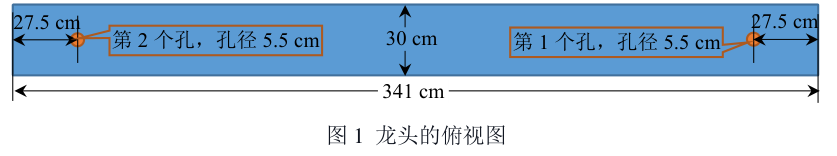
\includegraphics[width=\linewidth]{figures/dragon_statement_fig1.png}
  \caption{Official statement figure (cropped from the CUMCM 2024 A PDF) delivered to the agent.}
  \label{fig:dragon}
\end{subfigure}
\hfill
\begin{subfigure}{0.56\textwidth}
  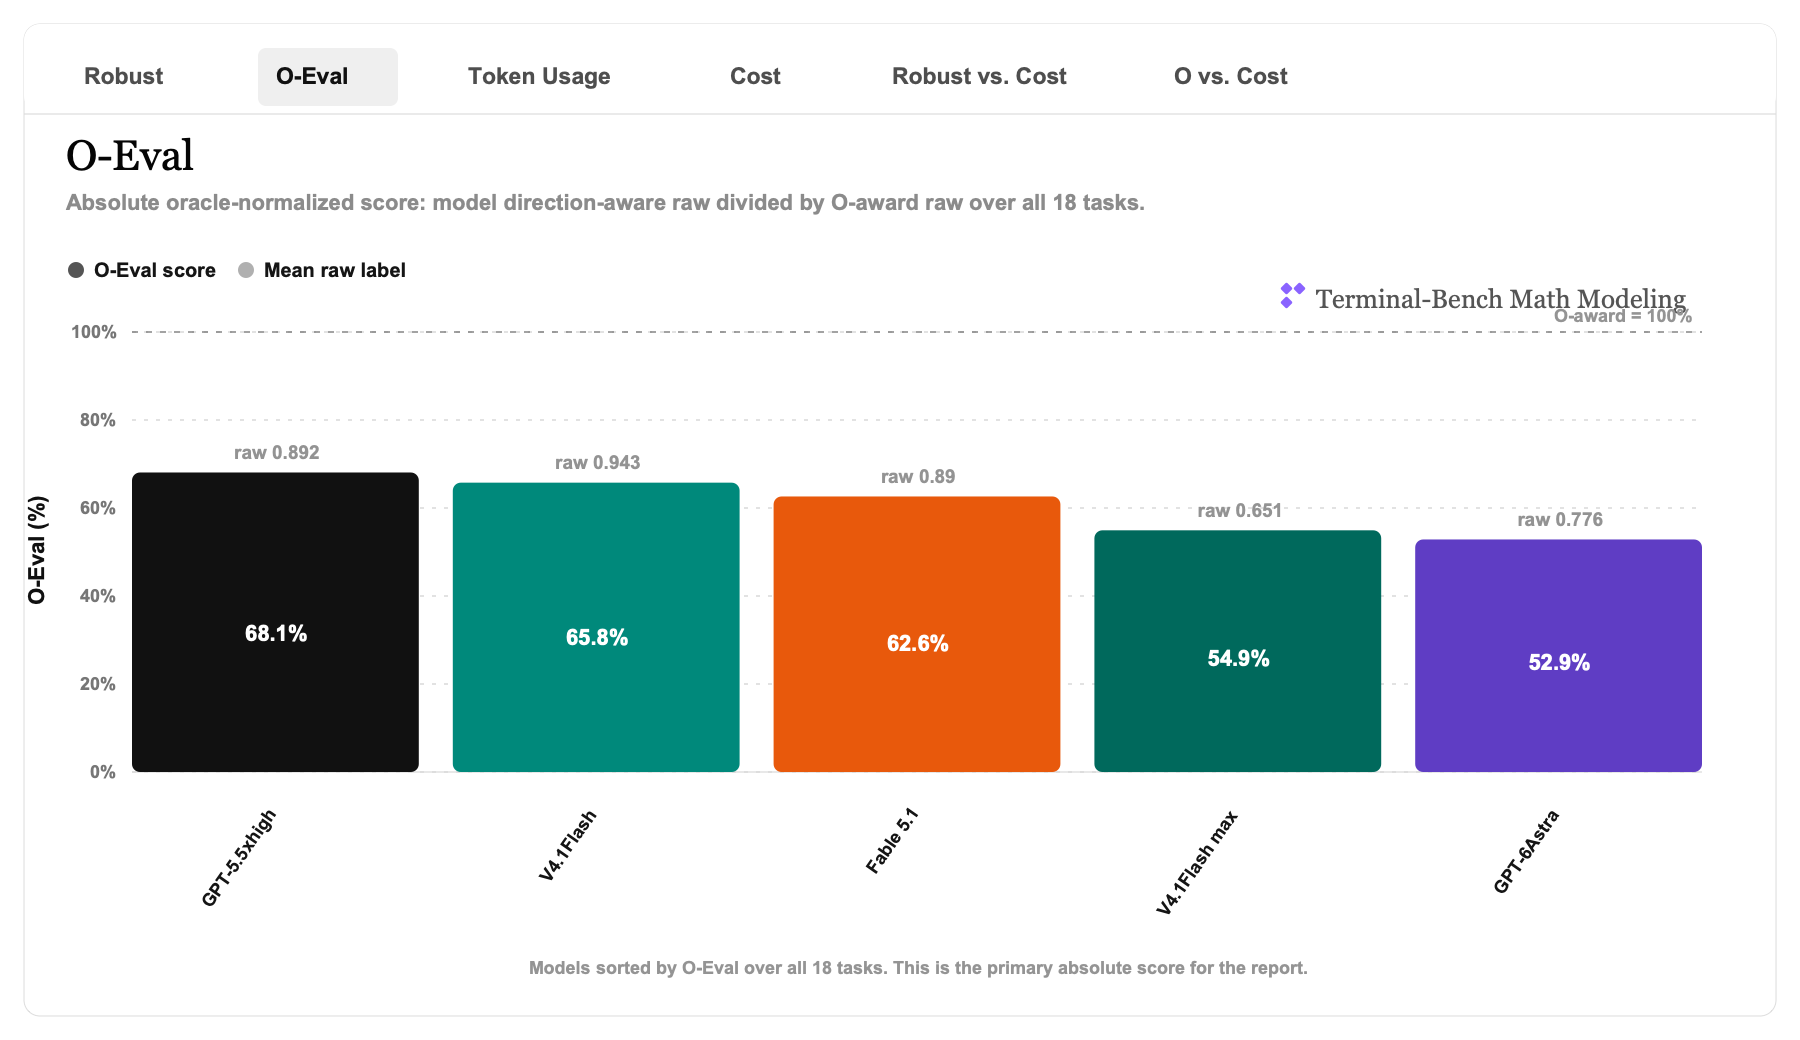
\includegraphics[width=\linewidth]{figures/mm-o-eval-bar.png}
  \caption{\oeval{} for the multimodal subset.}
  \label{fig:bar}
\end{subfigure}
\caption{Left: an official statement figure, cropped from the source PDF and delivered inline in the prompt---one of the 21 load-bearing figures. Right: the multimodal \oeval{} board.}
\label{fig:teaser}
\end{figure}
